% This is samplepaper.tex, a sample chapter demonstrating the
% LLNCS macro package for Springer Computer Science proceedings;
% Version 2.20 of 2017/10/04
%
\documentclass[runningheads, twocolumn]{llncs}
%
\usepackage{graphicx}
\usepackage{amsfonts,amssymb}
\usepackage{amsmath}
\usepackage{multirow}
\usepackage{bigstrut}
\usepackage{booktabs}
\usepackage[backref]{hyperref}
\usepackage{geometry}
\geometry{a4paper,scale=0.8}

% Used for displaying a sample figure. If possible, figure files should
% be included in EPS format.
%
% If you use the hyperref package, please uncomment the following line
% to display URLs in blue roman font according to Springer's eBook style:
% \renewcommand\UrlFont{\color{blue}\rmfamily}

\begin{document}
%
\title{Transformer Based Memory Network for Sentiment Analysis of Chinese Weibo Texts}
\titlerunning{Sentiment Analysis of Chinese Webo Texts based TF-MN}
%
%\titlerunning{Abbreviated paper title}
% If the paper title is too long for the running head, you can set
% an abbreviated paper title here
%
\author{Jiang Ming\inst{1}\and
Junlei Wu\inst{2}\and
Min Zhang\inst{3}}
%
\authorrunning{Jiang. et al.}
% First names are abbreviated in the running head.
% If there are more than two authors, 'et al.' is used.
%
\institute{Institute of Software and Intelligent Technology, Hangzhou Dianzi University, Hangzhou 310018, China\\
\email{jmzju@163.com}, \email{171050047@hdu.edu.cn}, \email{hz\_andy@163.com}}
%
\maketitle              % typeset the header of the contribution
%
\begin{abstract}
Weibo has already become the main platform of mobile social and information exchange. Therefore, the sentiment feature extraction of Weibo texts is of great significance, and aspect-based sentiment analysis (ABSA) is useful to retrieval the sentiment feature from Weibo texts. Now, context-dependent sentiment feature is obtained by widely using long short-term memory (LSTM) or Gated Recurrent Unit (GRU) network, and target vector is usually replaced by average target vector. However, Weibo texts has become increasingly complex and feature extraction with LSTM or GRU might cause the loss of key sentiment information. Meanwhile, average target vector might be wrong target feature. To correct drawbacks of the old method, a new Transformer (a new neural network architecture based on self-attention mechanism) based memory network (TF-MN), is introduced. In TF-MN, the task is migrated into question answering process in which context, question and memory module is modified optimally. The text is encoded by Transformer in context module, question module transfer target into sentiment question, memory module eliminates the effect of unrelated words by several extractions. The result of the experiment proves that our model reaches better accuary than the state-of-the-art model.

\keywords{ABSA  \and Transformer \and Memory Network \and Weibo texts.}
\end{abstract}
%
%
%
\section{Introduction}
Recently, rapid development has been witnessed in mobile social which has fully infiltrated into the global user communities. As one of the most important mobile social applications, Weibo contains entertainment, social, marketing, food and so on~\cite{DBLP:conf/IEEEcit/ChenLZW16}. It has gradually evolved from a social demand that satisfies people’s “weak relationship” to a popular public opinion platform, becoming one of the most important realtime information sources and the center of spreading public opinion. Viewpoints and proposals in Weibo are universal and adaptive due to large amounts of users along with the differences of their standpoints and knowledge they have. By performing sentiment analysis on the content published by Weibo users, it can restore the real emotions of users as much as possible, help people to get hot topics in time, help control the direction of public opinion, and help to analyze product reviews. This sentiment analysis technology not only assists users in optimizing their purchasing decisions, but also helps them to self-improve, improve market competitiveness, and accurately discover and exploit the hidden business and social values in Weibo.

Weibo sentiment analysis refers to judging the emotional tendency by analyzing and mining subjective information in Weibo. At present, there are many studies on the emotional analysis of Weibo in China. According to the granularity, it can be divided into fine-grained sentiment analysis and coarse-grained sentiment analysis. The coarse-grained sentiment analysis is mainly based on the text level and the sentence level, and only the emotional words are considered in the analysis process, and the emotions of the evaluation object and its attributes are not considered; Fine-grained sentiment analysis generally refers to lexical-level sentiment analysis.

In this paper, we use aspect level sentiment analysis(ABSA), a fine-grained sentiment analysis technology, to process Weibo texts. A piece of Weibo text may contains many aspects, each of which expresses a variety of emotions. For example, the text, “Nice Service but the food was too bad!”, expresses the emotions of two different goals. With the approach of aspect level sentiment analysis, we can analyze the opinions and emotions expressed by Weibo in a more fine-grained manner. As to the above instance, we analyze the emotions to be expressed in this text from two aspects. The polarity is positive when target is “service”, but it turns negative if “food” is seen as target. This hierarchical analysis method is very effective for digging deep into the emotions expressed by a piece of text.

In terms of sentiment classification, whether it is coarse-grained or fine-grained sentiment analysis, the methods used can be divided into three categories, supervised machine learning methods, unsupervised sentiment analysis methods, and semi-supervised sentiment analysis methods.

Supervised machine learning methods perform supervised training and testing through classifiers by selecting emotional classification features such as emotional words. The milestone is that Pang et al. applied three representative classifiers (support vector machine SVM, naive Bayes NB, maximum entropy ME) to classify the text emotionally~\cite{DBLP:conf/emnlp/PangLV02}.Some scholars compare different classification algorithms. Yanxia Yang used Bayesian algorithm and SVM classification algorithm to analyze the sentiment of Weibo, and compared the advantages and disadvantages of the two algorithms in classification performance, showed that Bayesian algorithm works better~\cite{yang2015microblog}. Some scholars have improved the classification algorithm to make the classification better. Chen Bingfeng et al. improved the Linear-chain CRF model and proposed a two-layer CRF model, which can better satisfy the car entity's recognition of emotional entities and emotional tendency classification needs~\cite{Chen2017A}.

The semi-supervised analysis method is based on a small number of labeled data sets, and the size of the labeled data set is expanded by testing some unlabeled data. Repeat the previous steps to predict the data step by step. Xiaoguang Zhu combined the existing annotation set with the active learning method in semi-supervised learning to mark the emotional polarity and category of Weibo text, to reduce the cost of labeling, and apply the labeled data set to supervised learning~\cite{zhu2013chinese}.

Unsupervised sentiment analysis methods are based primarily on existing sentiment lexicons or the existing emotional dictionary which is expanded to perform sentiment analysis on the text. Currently, it is representative and widely used in dictionary resources. The English language mainly includes WordNet and General Inquirer. Emotional dictionaries commonly used in Chinese are "HowNet", NTUSD, C-LIWC, DUTIR, etc.

Since supervised learning relies on sufficient annotated corpus, Weibo, such a large amount of Internet text, leads to manual inability to label large-scale corpora, and its scope and scale are limited. In addition, Weibo contains too much uncertainty, the unsupervised method of constructing an emotional dictionary cannot cover all emotions.  Unlike traditional machine learning methods, I combine semi-supervised learning with neural network learning method. A small set of annotation training sets is provided to predict the sentiment classification of unlabeled data sets.

Learning text features is important for neural network learning methods. Learning text feature is mainly by means of sequence transduction models in neural network models. The mainstream of sequence transduction models are based on complicated recurrent neural network (RNN) or convolutional neural networks (CNN) which consist of an encoder and a decoder. The models that connect the encoder and decoder through attention cells give the best combined properties~\cite{DBLP:conf/nips/VaswaniSPUJGKP17}. Long short-term memory (LSTM)~\cite{DBLP:journals/neco/HochreiterS97} and gated recurrent (GRU)~\cite{DBLP:journals/corr/ChungGCB14} neural networks have been attained the best result in sentiment analysis domain. However, Weibo texts has become increasingly complex and it is quite difficult to extract context-dependent text feature. LSTM and GRU are the best sequence transduction models at present, which can’t process long text. Reference~\cite{DBLP:conf/naacl/SongSLZ18} puts forward that text could be separated into four parts to ensure no key information lost. But, context-dependent text feature may be unable to be extracted.

Besides, target may consist of several words, and target feature can be learned directly by sequence transduction models. Experiment shows that average target vector is the best method to get target feature~\cite{DBLP:journals/eswa/DoPMA19}, however this method has certain weaknesses. For example, in text “Nice macarons in France are not good at all.”, the target is “Nice macarons”, consists of two words. Due to the limited number of words, vocabulary only contains “Nice”, and thereby “macarons” will be assigned to a set of minimal random feature. Then, the average target feature of “Nice macarons” equals approximately the feature of “Nice”, which leads to wrong results of classification.

Based on the two problems analyzed above, we propose a memory network model that combines Transformer. Transformer is a novel network architecture, based solely on attention mechanisms without recurrent and convolutional structure entirely. Its basic unit is self-attention mechanism which can obtain better context-dependent text representation using interactive calculation in each part of sequence whether the size of sequence.

And we utilize the memory network to capture sentiment information of given target. It contains four modules: the context module for encoding Weibo texts, the question module for storing knowledge from previous steps, the question module for conversion target and encoding questions, and the answer module for evaluating sentiment polarity by data from memory module.

The memory network is proposed for the question answering task, however, the aspect-based sentiment classification doesn’t have an exact question. The original MN handles this by initializing the problem vector generated by the problem module with a zero or offset vector, while we argue that every target in the text could be converted into a question. We propose the Transformer based memory network (TF-MN) to realize our ideas, the question module of TF-MN treats each target in the text as implicitly asking a question “What is the emotion tendency of target in the text?”. Figure~\ref{TF-MN} is the overview of TF-MN architecture.

\begin{figure}[htb]
	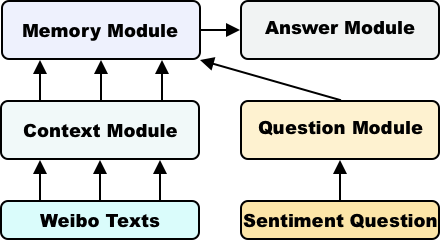
\includegraphics[width=0.4\textwidth]{TF-MN.png}
	\centering
	\caption{The architecture diagram of TF-MN.}\label{TF-MN}
\end{figure}

 The following is a summary of our work:

\begin{itemize}
	\item[$\vcenter{\hbox{\tiny$\bullet$}}$] In sentiment analysis task, we extract long text feature by using Transformer for the first time. Our model effectively solves the problem of inaccurate long text feature extraction by using LSTM and GRU.
	\item[$\vcenter{\hbox{\tiny$\bullet$}}$] The question module does not average the target word vector, but is responsible for designing the corresponding target problem to handle the case where the target consists of multiple words.
	\item[$\vcenter{\hbox{\tiny$\bullet$}}$] On our dataset, our model achieved the best accuracy, and the experimental results further show that using Transformer and adding implicit question can actually improve the performance of the model.
\end{itemize}

\section{Related Work}
ABSA is a subdomain in sentiment analysis which focuses on fine-grained sentiment information~\cite{DBLP:series/synthesis/2012Liu}. There are two main approaches to solve ABSA problem.

The first one is the traditional method using lexicons and rules. The extracted features are used to train sentiment classifiers like SVM. However, the performance of these methods is often highly dependent on the quality of the manual features. In addition, designing these features is labor intensive. Reference~\cite{DBLP:conf/kdd/HuL04} compute sentiment word score using the weight sum method. Reference~\cite{DBLP:conf/wsdm/DingLY08} proposed a holistic lexicon-based method involving both explicit and implicit opinions. The method improves performance to identify the aspect level relations by multiple kernels ~\cite{DBLP:conf/cicling/NguyenS15}.

The second one is the machine learning method. Reference~\cite{DBLP:conf/acl/RameshKFG15} developed a weakly supervised joint model for the emotional aspects of online courses, using a recently developed extensible statistical relationship model called hinge loss Markov random field to model the relationship between aspects and emotions. And it employed hingeloss Markov random fields to tackle ABSA in MOOC. Reference~\cite{DBLP:conf/emnlp/WangE14} present an emotionally consistent topic model (SATM) in which it combine two types of external knowledge: the productlevel overall rating distribution and the wordlevel sentiment dictionary. It put forward a emotion-aligned model for to predict aspect rate. Reference~\cite{DBLP:conf/semeval/KiritchenkoZCM14} combined vocabulary-based method and characteristics-based Support Vector Machine (SVM), and  detect sentiment towards aspect words in SemEval 14 competition at first time. It first detects the emotional aspects of the category, the third test term, the first and second emotions that detect terminology in the field of laptops and restaurants. 

Reference~\cite{DBLP:conf/emnlp/NguyenS15} constructed binary phrase dependency tree of target to build the feature of aspect words. It presents a new approach to identifying emotions in terms of entities. It is an extension of RNN (Recursive Neural Network) that takes into account the dependency and composition of sentences. Reference~\cite{DBLP:conf/coling/TangQFL16} developed two target-related long-term short-term memory (LSTM) models in which target information is automatically considered. The way we evaluate benchmark data sets on Twitter. It solved the problem using recurrent neural network, and suggested two approaches TD-LSTM and TC-LSTM. Reference~\cite{DBLP:conf/emnlp/WangHZZ16} proposed a long-term short-term memory network based on attention for aspect-level emotional classification. When different aspects are used as input, the attention mechanism can be concentrated in different parts of the sentence.

 Reference~\cite{DBLP:conf/emnlp/TangQL16} introduced a deep memory network method to solve ABSA task. It used hierarchical structure model in which the text was fully connected with target for final classification by using attention cell~\cite{DBLP:conf/cikm/ChengZZKZW17}. Based on this series of studies, reference~\cite{DBLP:conf/coling/HeLND18} propose two new methods to improve attention. First, it propose a target representation method that can better capture the semantics of the opinion target. Second, it introduce a attention model that incorporates syntactic information into the attention mechanism. it experimented with the attention-based LSTM (long-short-term memory) model using SemEval's 2014, 2015, and 2016 data sets. Although it uses local attention to use syntactic information, the proposed method is different from the local attention used in itself. It uses local attention to select words within a larger window to maintain semantic integrity, but the local attention used in the proposed method tends to small window size to capture relatively pure emotional information about the target. In addition, it uses distance weights in local attention to highlight words that are closer to the target, and the proposed method uses a gating mechanism to dynamically re-weight the words in the sentence. More importantly, compared to itself, the proposed method uses local and global attention to generate the final sentence representation, which can make up for the missing information of local attention and is more robust to parsing errors.
 
 Reference~\cite{DBLP:journals/corr/abs-1802-00892} introduced a method of dividing each sentence into three parts, and the context-dependent feature was extracted using bidirectional GRU. LSTM and GRU are widely used by the models mentioned above without considering how to extract the long text feature. Meanwhile, they never consider the situation of lacking target in vocabulary when getting target by average target vector.

Different from the above model, we mainly carry out emotional classification from three aspects: optimizing feature extraction; transforming the form of target vector; eliminating the influence of irrelevant emotional words. 

First of all, when we use LSTM to process text features, we find that when LSTM processes long text (more than 50 words), the gradient disappears. For this problem, we are inspired by the self-attention mechanism. Based on Transformer, the best-performing self-attention model, we use it to solve the forgotten information of serialized models such as lstm. 

Secondly, we find that it has been a mistake to use the average vector instead of the target. In order to solve this problem, we try to convert this target vector into a form that is transformed into an emotional problem. The results show that emotional questions are more able to express the characteristics of the target. 

Thirdly, we observed that there are some emotional words in the data set that are not related to expressing emotions. We believe that these unrelated emotional words will mislead the results of the experiment. Therefore, we use the memory network to eliminate the influence of unrelated emotional words on the classification results by extracting emotional features multiple times. The effect of classification has improved, indicating that the memory network can eliminate the influence of emotionally unrelated words. 

We ran the other models mentioned above on our dataset. The experimental results show that our model is better than the best model in our data, indicating the superiority of our model.

\section{The comparison of Sequence Transduction and Self-Attention model}

\begin{figure*}[htb]
	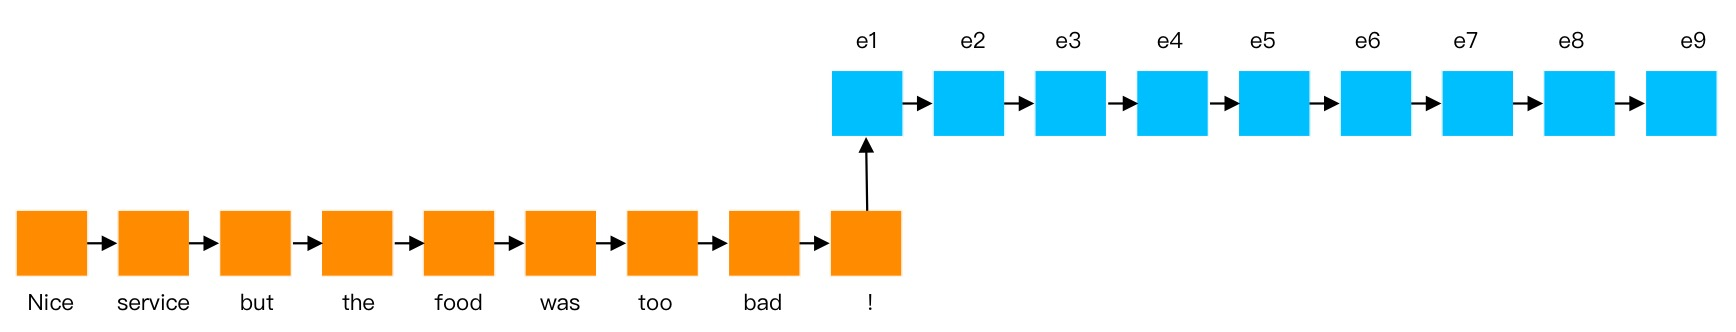
\includegraphics[width=\textwidth]{rnn4.jpg}
	\centering
	\caption{The architecture of sequence transduction model.}\label{seq2seq}
\end{figure*}
The first thing to know is that the sequence transduction model architecture is like this Fig.~\ref{seq2seq} before the attention mechanism emerges. First, the sequence model will input the text into the encoder(the blue part of the Fig.~\ref{seq2seq}), process it according to the order of the text, and get a feature representation of the input text. Then the decoder outputs the feature as a feature representation of a fixed shape. The blue part of the Fig~\ref{seq2seq} is the output of sequence transduction model. However, this way of transmitting information leads to a large loss of information, especially long sentences and language pairs with different word order, such as Fig.~\ref{seq2seq}.

It can be found that to translate "nice" into the feature vector of $e_1$, it must go through a long distance, which may be mixed with noise or lose some useful information, so it is difficult to extract accurate text features. Even after the addition of a partial attention mechanism to assist in the extraction of text features, extraction errors can occur. The reason is the insufficient capture of the relationship. In the feature extraction task of texts, we need to discover three kinds of relationships: the relationship inside the source sentence; the relationship inside the target sentence; the relationship between the source sentence and the target sentence.

Even if the above sequence transduction model uses the attention mechanism to capture the relationship between the source and target sentences, but still uses RNN to capture the relationship between the internal and the target sentences. The model captures the relationship from side to side (better with bidirectional sequence), but this is not straightforward, especially for some distant distances.

In addition to the lack of learning long-distance relationships, seq2seq has one drawback: training slowly. Because it it takes a word to look from left to right one by one, which makes RNN not take advantage of the parallel computing power of the GPU like CNN.

\begin{figure*}[htb]
	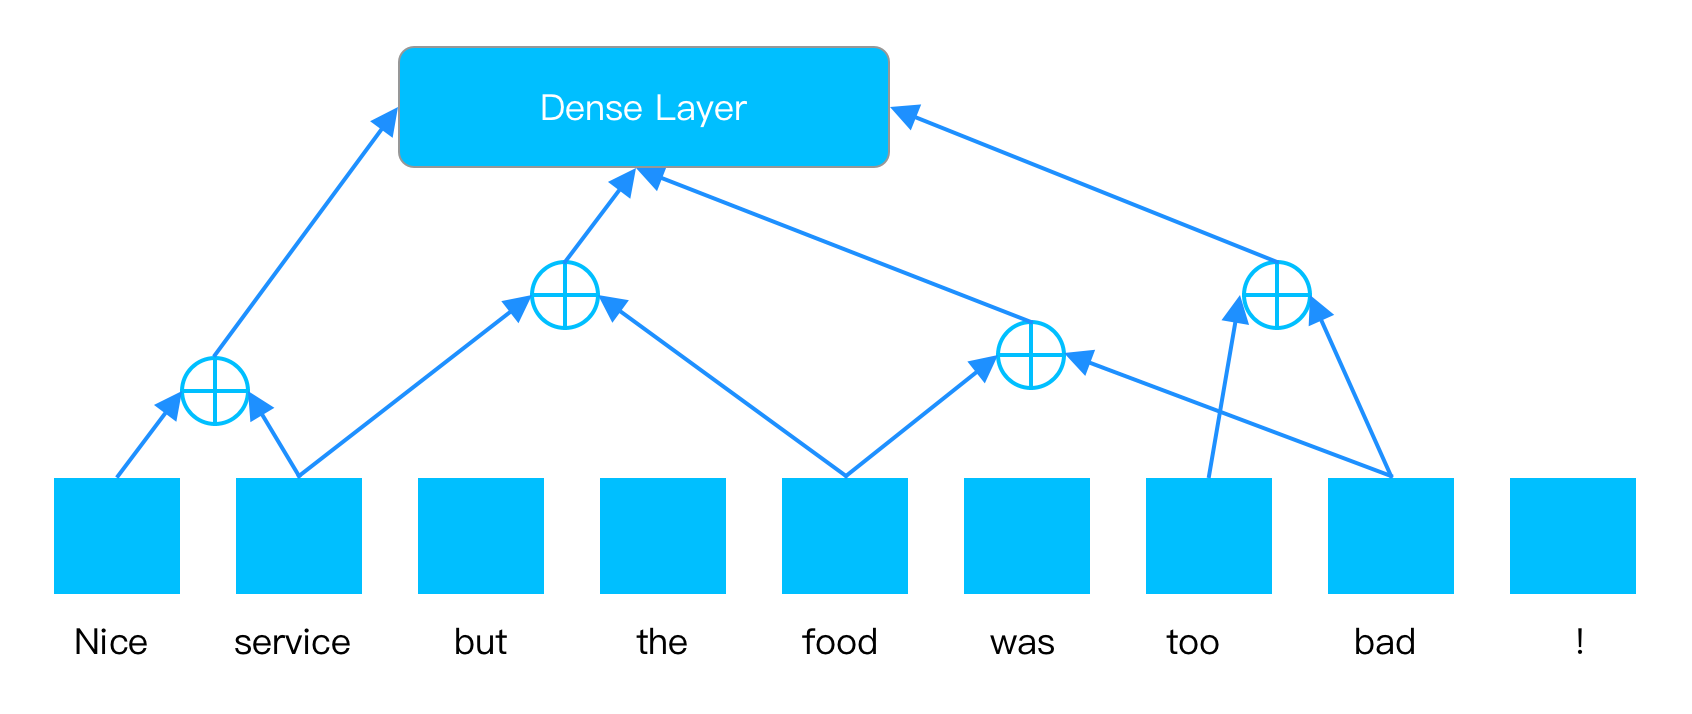
\includegraphics[width=0.6\textwidth]{self-attention2.png}
	\centering
	\caption{The architecture of self-attetion model.}\label{self-attention}
\end{figure*}

In order to solve the shortcomings of the sequence transduction model, we need to use a novel architecture, the self-attention mechanism, whose model structure is as shown in the Fig.~\ref{self-attention}. 

Fig.~\ref{self-attention} is a simple self-attention mechanism framework. We can see that each word in the sentence is correlated (for the sake of drawing, we omit the connection of some words). Therefore, the self-attention mechanism can achieve long-distance dependence and solve the problem of gradient disappearance. And this calculation method has no sequence requirements, it can be operated in parallel, saving a lot of time.

\begin{figure*}[htb]
	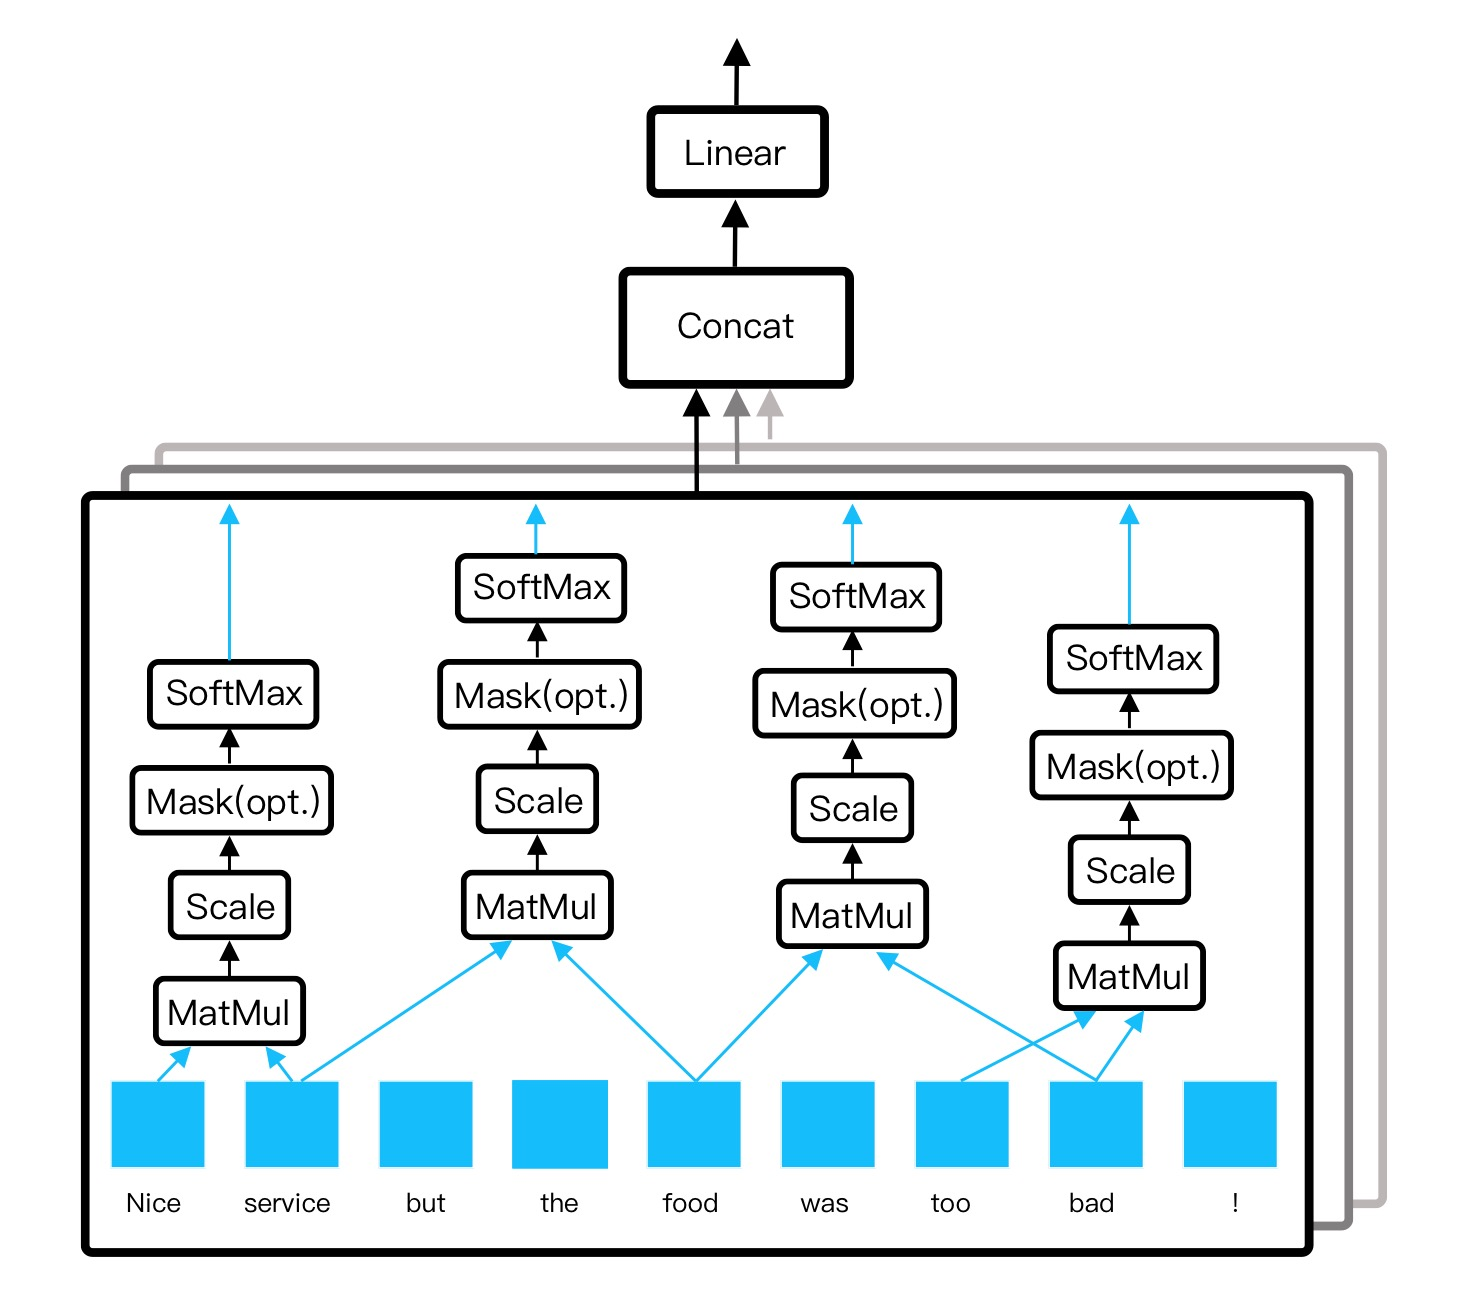
\includegraphics[width=0.7\textwidth]{transformer.jpg}
	\centering
	\caption{The architecture of transformer-self-attention model.}\label{transfromer}
\end{figure*}

Fig.~\ref{transfromer} is a Transformer self-attention model architecture diagram, which is also based on a self-attention mechanism, except that it is more complex than Fig.~\ref{self-attention}. It mainly performs the deformation and softmax operations on the results of the association calculation of each word, and finally combines the results of each round of the self-attention mechanism to obtain a more comprehensive text feature representation.

The calculation process of Fig.~\ref{transfromer}'s self-attention mechanism can be expressed as the following formula:
\begin{equation}
Attention(e_i, e_{i+1})=softmax(\dfrac{e_i e_{1+1}^T}{\sqrt{d_k}})
\end{equation}
\begin{equation}
head_i=Attention(e_i, e_{i+1})
\end{equation}
\begin{equation}
MultiHead(e_i, e_{i+1})=Concat(head_i)W^O
\end{equation}
where $e_i$ represents a word, $d_k$ represents the dimension of the word vector, and $W^O$ is a randomly generated parameter matrix.

I think the biggest improvement of transformer relative to the traditional sequence transduction is:

\begin{itemize}
	\item[$\vcenter{\hbox{\tiny$\bullet$}}$] Propose to use the attention mechanism to directly learn the internal relationship of the source language and the internal relationship of the target language, instead of learning with RNN as before;
	\item[$\vcenter{\hbox{\tiny$\bullet$}}$] A multi-head attention mechanism is proposed for the assumption that there are many different relationships, which is somewhat similar to the concept of multi-channel in CNN;
	\item[$\vcenter{\hbox{\tiny$\bullet$}}$] The position of the word is encoded by the sin and cos functions of different frequencies.
\end{itemize}

\section{The Proposed Model}
We presents TF-MN model for ABSA in this section. The task of ABSA concluded as follows: given a text consisting of \emph{n} words $C = \{w_1^C, w_2^C, \cdots, w_{n-1}^C, w_n^C\}$ that is named context, a target $T = \{w_1^T, w_2^T, \cdots, w_{i-1}^T, w_i^T\}$ in which sereval adjacent words appear in the context, and the aim is predicting the sentiment polarity of the specified target in the given context.

\begin{figure*}[htb]
	\includegraphics[width=0.95\textwidth]{Transformer-mn.png}
	\centering
	\caption{The architecture of TF-MN model.}\label{Transformer-mn}
\end{figure*}

Fig.~\ref{Transformer-mn} shows the TF-MN architecture, which converts context into a consecutive low dimensional sequence with pretrained word embeddings in the context module. And Transformer processes context sequence to preserve sequential information in memory module. In question module, target is converted into sentiment question. The question is in the form of “What is the emotion tendency of target in the text?”. Then, Transformer is also operated upon the question. In memory module, we eliminates the effect of unrelated words by several extractions. Finally, softmax layer outputs sentiment polarity. Each step of our model are showed as follows.

\subsection{Context Module}
The context module includes the following layers: the context encoder, the location encoder and the fusion layer. The context and the location encoder layer encode each context and location information into a vector separately, while the fusion layer exchange information between these encoded vectors using Transformer.

\subsubsection{Context encoder layer}
Specified a context  $C = \left\{w_1^C, w_2^C, \cdots, w_{n-1}^C, w_n^C\right\}$, every word in \emph{C} is converted into a \emph{k}-dimensional vector $e_i^C \in \mathbb{R}^k$ with a pretrained word embedding matrix $E \in \mathbb{R}^{k\ast\left|V\right|}$, such as Tencent AI Lab Embedding~\cite{DBLP:conf/naacl/SongSLZ18}:
\begin{equation}
e_i^C = E(w_i^C)
\end{equation}
where “$\left|V\right|$, \emph{k}" are the size of vocabulary and word vector respectively.

\subsubsection{Location encoder layer}
We establish a context location word embedding matrix  $L = \in \mathbb{R}^{k\ast n}$, which maps word location into a \emph{k}-dimensional vector $l_i^C \in \mathbb{R}^k$:
\begin{equation}
	l_i^C = L(w_i^C)
\end{equation}
where \emph{n} is the dimension of row vector in \emph{L}. To provide rich location information for context, row vector of \emph{L} is a \emph{k}-dimensional vector consisting of \emph{k} location information. Matrix \emph{L} is a set of parameters to be trained, in which every row vector will be assigned a sequence of location information with random normal $U\left(-0.02, 0.02\right)$.

\subsubsection{Fusion Layer}
The fusion layer processes the context vector $E_C$ and context location vector $L_C$ which contain exchanged information among vectors. We generate context representation $H_C \in \mathbb{R}^{k\ast nc}$:
\begin{equation}
	H_c = Transformer(E_C, L_C)
\end{equation}
where \emph{nc} denotes the max size of context (If the length is not enough, fill it with 0).

\subsection{Question Module}
The question module further also contains these layers: the question encoder layer, the location encoder layer and the fusion layer. The question encoder layer converts target into sentiment question firstly, and then encodes question into vector. The location encoder layer encodes location information into a vector. The fusion layer fuses these vectors into more specific features through the Transformer.

\subsubsection{Question encoder layer}
Given a question $T = \left\{w_1^T, w_2^T, \cdots, w_i^T\right\}$,  \emph{T} consists of one or more words, which can be included in \emph{C} or doesn’t appear in \emph{C}. If \emph{T} is embedded in sentiment question, you will get the question as “What is the emotion tendency of target in the text?”. Every word in question is converted into a \emph{k}-dimensional vector $e_i^Q \in \mathbb{R}^k$ with a pretrained word embedding matrix \emph{E}:
\begin{equation}
	e_i^Q = E(w_i^Q)
\end{equation}

\subsubsection{Location encoder layer}
We also establish a question location word embedding matrix \emph{L}, which maps word location into a \emph{k}-dimensional vector $l_i^Q \in \mathbb{R}^k$:
\begin{equation}
	l_i^Q = L\left(w_i^Q\right)
\end{equation}
where the location information matrix of \emph{Q} is the same as context module.

\subsubsection{Fusion layer}
The fusion layer generates the sentiment question representation $H_Q \in \mathbb{R}^{k\ast nq}$:
\begin{equation}
	H_Q = Transformer\left(E_Q, L_Q\right)\label{H_Q}
\end{equation}
where \emph{nq} denotes the max size of question.

\subsection{Memory Module}
The memory module has three components: the attention gate, feature conversion and the memory update gate, which is used to combine information from context with target and purify of the target vector from the given context.

The output \emph{F} from context module, the question $q^\ast$ from question module and the acquired knowledge stored in the memory vector $m_{t-1}$ from the previous step.

The three inputs are transformed by:
\begin{equation}
	u = \left[F \ast q^\ast; \left|F - q^\ast\right|; F \ast m_{t-1}; \left|F - m_{t-1} \right|\right]\label{con:attentiongate}
\end{equation}
where “;” is concatenation. “ $\ast$,$-$,$\left|\right|$ ”are element-wise product, subtraction and absolute value respectively. \emph{F} is a matrix of size $\left(1, H_C\right)$, while $q^\ast$ and $m_{t-1}$ are vectors of size $\left(1, H_Q\right)$ and $\left(1, H_m\right)$, where $H_m$ is the output size of the memory update gate. To allow element-wise operation, $H_C$, $H_Q$ and $H_m$ are set to the same shape. In equation~\eqref{con:attentiongate}, the first two terms measure the similarity and difference between facts and the question. The last two terms have the same functionality for context and the last memory state.

Let the \emph{i}-th element in $\alpha$ to be the attention weight for $w_i^C$. $\alpha$ is obtained by transforming \emph{u} using a two-layer perceptron:
\begin{equation}
	\alpha = softmax\left(tanh\left(u\cdot W_{m1}\right)\cdot W_{m2}\right)
\end{equation}
where $W_{m1}$ and $W_{m2}$ are parameters of the perceptron and we omit bias terms.

The feature conversion takes \emph{F} and $\alpha$ as input and then get the updated \emph{F}:
\begin{equation}
	F = F \cdot \alpha\label{con:updatecontext}
\end{equation}

The memory update gate outputs the updated memory $m_t$ using question $q^{\ast}$, previous memory state $m_{t-1}$ and the updated \emph{F}: 
\begin{equation}
	m_t = relu\left(\left[q^\ast;m_{t-1};F\right]\cdot W_u\right)\label{con:updatememory}
\end{equation}
where $W_u$ is the parameter of the linear layer.

The memory module could be iterated several times with a new $\alpha$ generated for each time. This allows the model to attend to different parts of the facts in different iterations, which enables the model to perform complicated reasoning across sentences. The memory module produces $m_t$ as the output at the last iteration.

\subsection{Eliminate the effect  of Irrelevant Words}

\begin{figure*}[htb]
	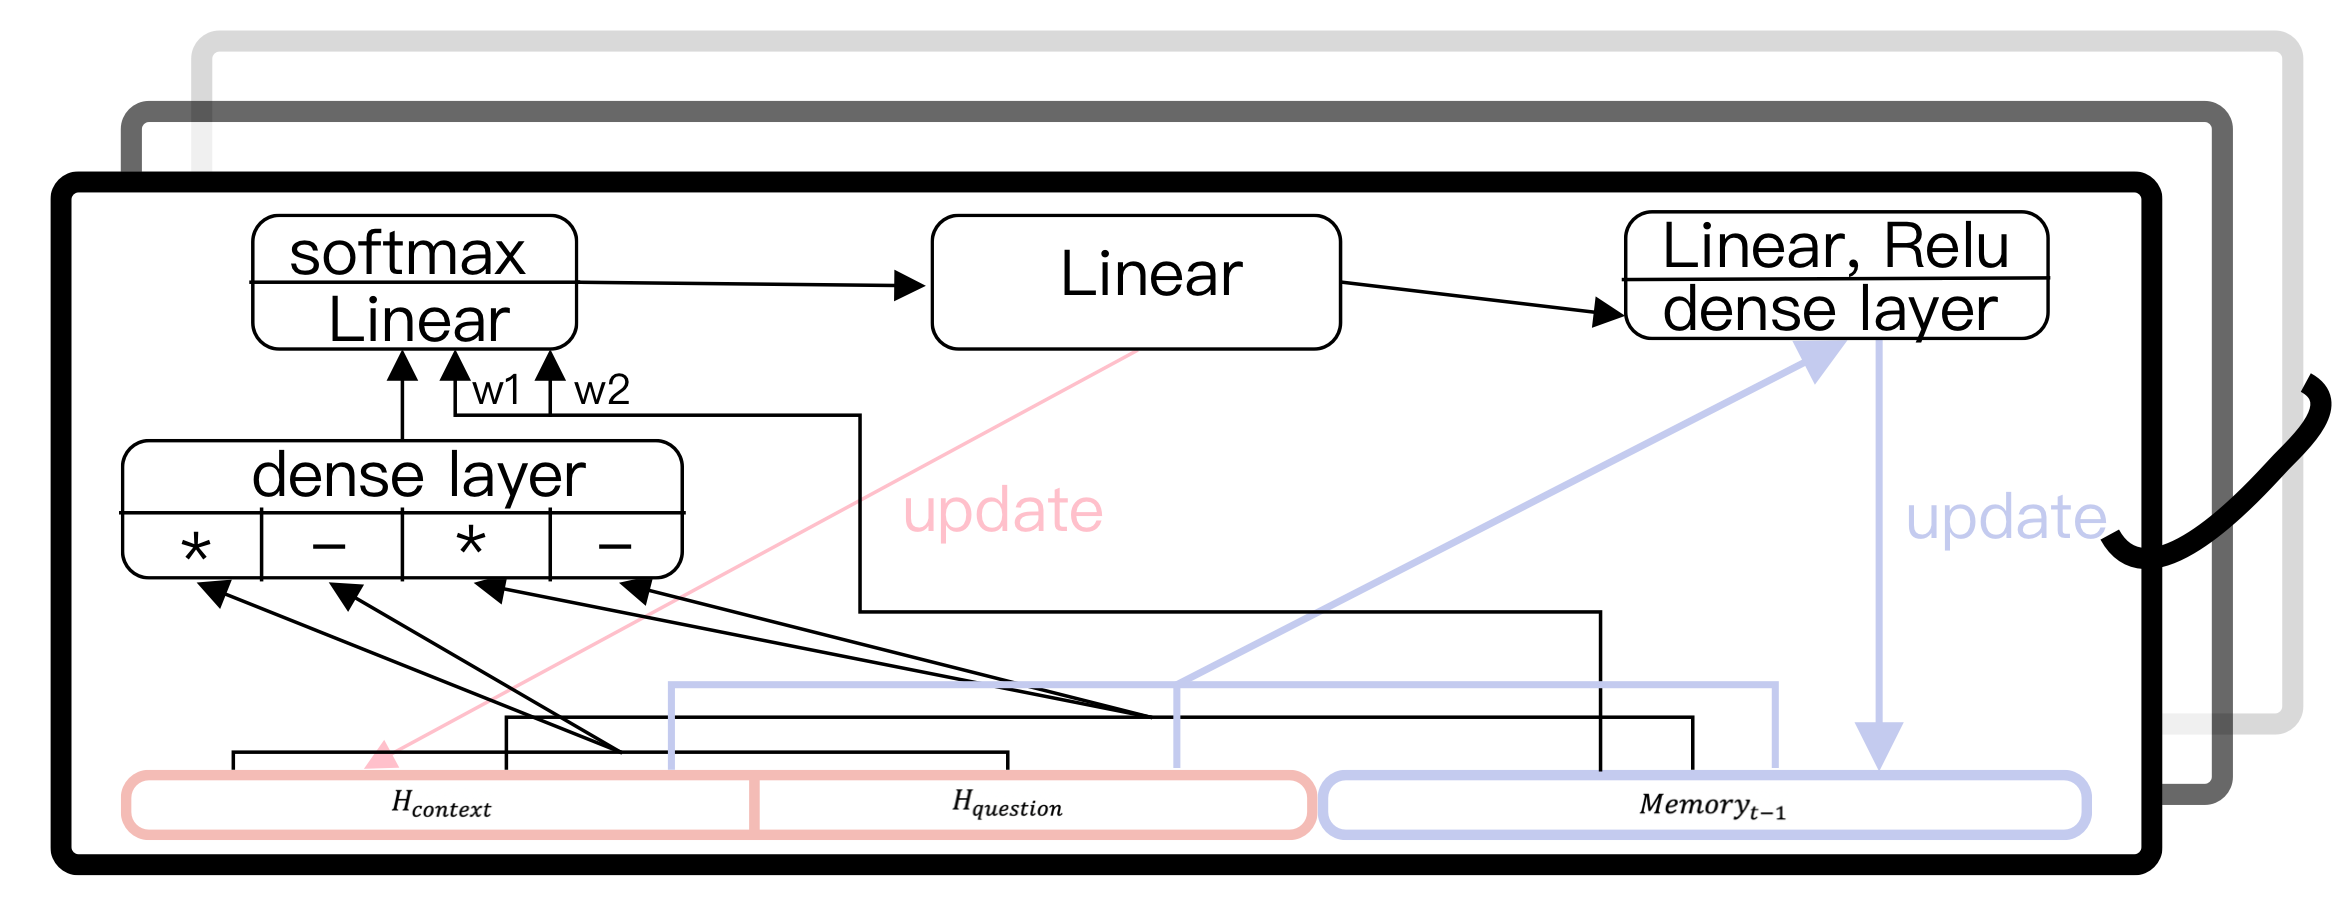
\includegraphics[width=0.9\textwidth]{memoryNetwork.png}
	\centering
	\caption{The architecture of memory network module.}\label{memorynetwork}
\end{figure*}

After introducing the composition of the above memory module, this section will carefully introduce the workflow of the memory module. This module is a very important part of my model, it is mainly used to eliminate the influence of unrelated emotional words in the text.
Fig.~\ref{memorynetwork}


\subsubsection{Attention Gate}
Formula~\ref{con:attentiongate} describes the calculation steps of the attention gate. First of all, the memory network has no memory. So we memory zero state $m_0$ equals H question. And perform multiplication and substraction between context and question  or between context and memory respectively, mark this result as D. Finally get attention gate by linear transformation of D and memory bias. Expressed as follows:
\begin{equation}
m_0 = H_{question}
\end{equation}
\begin{equation}
D_1 = [H_{context}*H_{question}; |H_{context}-H_{question}|]
\end{equation}
\begin{equation}
D_2 = [H_{context}*m_0; |H_{context}-m_0|]
\end{equation}
\begin{equation}
D = [D_1; D_2]
\end{equation}
\begin{equation}
AttentionGate = softmax(tanh(D\cdot m_0^1)\cdot m_0^2)
\end{equation}
where $m_0^1$ indicates the bias on the x-axis, and $m_0^2$ indicates the bias on the y-axis.

\subsubsection{Update Information}
And at this section, we update two parts of information: context and memory. Firstly we use linear transformation of context and attention gate to update context. Secondly we update memory by transformed context. 

Each time the context and memory information is updated, the weight of the unrelated emotional words will become smaller and smaller. By setting the number of iterations constantly, we set the impact of irrelevant emotional words to a minimum.

This update process can be described using the Formula~\ref{con:updatecontext} and Formula~\ref{con:updatememory}

\subsection{Answer Module}
In answer module, we regard the memory module outputs as the final representation, and put it into a softmax layer for aspect-based sentiment analysis task. To minimize the cross entropy error of sentiment classification, we train the model in a supervised method in which loss function is described as follows:
\begin{equation}
	loss = -\sum_{\left(c, q\right)\in T}\sum_{lb\in LB}P_{lb}^g\left(c, q\right)\cdot \log\left(P_{lb}\left(c, q\right)\right)
\end{equation}
where \emph{T} is all training items, \emph{LB} is the set of sentiment polatities, $\left(c, q\right)$ is a context-question pair. Our system outputs the probability of class \emph{lb} by computing the item $\left(c, q\right)$. $P_{lb}^g\left(c, q\right)$ means zero or one, expressing whether the item is positive or not. In the module, We calculate the gradients of the overall parameters by using back propagating and update them in a stochastic gradient descent manner.

\section{Experiment}

\subsection{Dataset and Experiment Setup}

\subsubsection{Dataset}
 In most recent ten years, a lot of Chinese Weibo competitions have been held, and many excellent datasets have been produced such as NLPCC 2013 and 2014 trainng dataset. Unfortunately, Most datasets only analyze the overall sentiment polarity of the entire sentence. So we try to construct a new dataset for ABSA. 
 
 We collect weibo data from Weibo, and each the weibo may contain multiple target entities. Each target can be an entity that appears in weibos or an abstracted entity in weibos. The emotional polarity of the goals we mark includes positive, negative, and neutral. If the target has a divergence between these three polarities, we will ignore this target entity. We mainly build dataset in the fields of restaurant which contains four aspects: traffic, service, price and environment. Then, we randomly selected 18480 Weibo items (a total of 22821 Weibo items) as training set, and the rest 4341 items as test set. In order to prevent the experiment from over-fitting, we set the number of entries for each sentiment class of the data to be the same. Table~\ref{stat-dataset} is the detail of the dataset. Finally, it is noted that the text length of our dataset is generally more than 200 words, which belong long texts. 

\renewcommand{\multirowsetup}{\centering}
\begin{table*}
	\caption{Statistics of dataset}
	\label{stat-dataset}
	\centering
	\scalebox{1.2}{
		\begin{tabular}{ccccc}
			\toprule[2pt]
			\textbf{type} & \textbf{aspect} & \textbf{negative} & \textbf{neutral} & \textbf{positive}\\
			\midrule[1pt]
			\multirow{2}{1in}{\textbf{train}} & 
			\textbf{traffic} & 629 & 629 & 629\\ & 
			\textbf{service} & 1929 & 1929 & 1929\\ &
			\textbf{price} & 2197 & 2097 & 2097\\ &
			\textbf{environment} & 1505 & 1505 & 1505\\
			\midrule[0.5pt]
			\multirow{2}{1in}{\textbf{test}} & 
			\textbf{traffic} & 88 & 88 & 88\\ & 
			\textbf{service} & 871 & 871 & 871\\ &
			\textbf{price} & 280 & 280 & 280\\ &
			\textbf{environment} & 208 & 208 & 208\\
			\bottomrule[2pt]
		\end{tabular}
	}
\end{table*}

\subsubsection{Evaluation}
We validate our model with the accuracy, and remove the label from test dataset before training the model. If the output label of the model answer module matches the label by manual method, it will become the right classification result.

\subsubsection{Parameter setting}
In the model, the word embeddings matrix of the contexts and targets in the dataset are assigned 200-dimensional vectors from Tencent AI Lab Embedding~\cite{DBLP:conf/naacl/SongSLZ18}. All words out of the vocabulary are randomly assigned a vector that obeys uniform distribution $U\left(-0.01, 0.01\right)$. To prevent data overfitting, we set the loss rate to 0.1. Our optimizer is Adam whose batch size and learning rate is 8 and 6.25e-5 respectively. We use jieba~\cite{sun2012jieba} to do Chinese phrase segmentation and generate the word vector matrix of our experiment. It is noted that the results of the experiment will change with each randomly assigned word vector even if we set up the seeds of the experiment. In order to solve this problem, the experimental data are obtained through average 10 experimental results.

\subsection{Experiment setting}
In order to test the performance of our model, we did the following set of experiments: SVM, LSTM, TD-LSTM~\cite{DBLP:conf/emnlp/WangHZZ16}, AT-LSTM\cite{DBLP:conf/emnlp/WangHZZ16}, IAN~\cite{DBLP:conf/ijcai/MaLZW17}, BILSTM-ATT, MENNET\cite{MENNET}.

Firstly, for the SVM experiment, we directly call the svm class inside sklearn~\cite{sklearn}. Then, since the number of samples is much larger than the number of features, we use a nonlinear kernel rbf. As for the optimal parameters of the model, we search for parameters in a large-range and large-step grid by the grid search method.

Secondly, we use the LSTM and BILSTM module in tensorflow, where we regard Webo text as input. Then, we output the results of the classification through the softmax layer.

Finally, we use the open source TD-LSTM and AT-lSTM~\cite{td-lstm_at-lstm}, IAN~\cite{IAN}, MENNET~\cite{MENNET} code on github to do experiment. Some parameters and settings of the experiment are as close as possible to the original author's paper.

\subsection{Model Comparisons and Analysis of Results}
In these models, SVM belongs to the traditional machine learning field; LSTM and TD-LSTM are general neural network model methods; AT-LSTM, IAN, BILSTM-ATT, MEMNET are mainly apply the attention mechanism.

 We compared the TF-MN model with the correctness of other models, and the results of this comparison are listed in Table~\ref{model-compare}. 
 
 In this table, we can observe that the performance difference between SVM performance and TF-MN model is the largest. We suggest it is caused by two reasons: the SVM training model does not use aspect; the SVM model only classifies the text, and does not mine deep text features. 
 
The effect of the LSTM model on this data set is also not very good, because LSTM can cause the loss of key sentiment information due to the mechanism of forget-door when processing long text.

The accuracy of TD-LSTM is much better than the single LSTM model because it combines ASPECT and text.

Unlike TD-LSTM, AT-LSTM uses a attention mechanism to effectively extract important emotional information from text with aspect, which greatly enhances the final classification result.

BILSTM-ATT is derived from the improvement of the AT-LSTM model, which uses a bidirectional LSTM model. Bidirectional LSTM can significantly improve the performance of the model for sequence classification problems.

The above models mainly focus on the impact of ASPECT on text, but the IAN model also uses the influence of text on ASPECT as a basis for classification. It believes that ASPECT and text should be mutually influential and not just one-way connections.

Based on the above models, MENNET proposes that the attention mechanism should directly affect the process of LSTM coding. Therefore, this model abandon the LSTM model and uses a simpler memory module to encode information. This memory model repeatedly uses the local attention mechanism to extract information and achieves good results.

Although MENNET is good enough, we found that the separate memory module does not encode the text information well during the experiment, and it is as bad as the LSTM model for longer text encoding. At the same time, we also feel that the previous treatment of ASPECT is too rough. Based on these two problems, we improve the MENNET model and achieve better model results.

\begin{table}
	\caption{3-way experimental results in accuracy. 3-way represents the three polarities of posi-tive, negative, neutral. Best scores in each group are in bold.}
	\label{model-compare}
	\centering
	\scalebox{1.2}{
		\begin{tabular}{ccc}
	    \toprule[2pt]
		\textbf{model} & \textbf{3-way restaurant}\\
		\midrule[1pt]
		\textbf{SVM} & 51.55\\
		\textbf{LSTM} & 52.45\\ 
		\textbf{TD-LSTM} & 55.26\\
		\textbf{AT-LSTM} & 56.34\\
		\textbf{BILSTM-ATT} & 57.47\\
		\textbf{IAN} & 58.33\\
		\textbf{MEMNET} & 60.78\\
		\textbf{TF-MN} & \textbf{61.67}\\
		\bottomrule[2pt]
	\end{tabular}
}
\end{table}

\subsection{Memory Network Optimization}

To improve the effect of the memory module to extract emotional information, we conducted a number of experiments to optimize and adjust the number of our memory updates. We found that when the updated hop count is set to 5, the model classification works best. The results of these groups of experiments are shown in table~\ref{hop-compare}. We believe this is due to excessive update operations that cause the local attention mechanism to repeatedly operate on the same block of text.

\begin{table}
	\caption{The result of Memory network hop count comparison.}
	\label{hop-compare}
	\centering
	\scalebox{1.2}{
		\begin{tabular}{ccc}
			\toprule[2pt]
			\textbf{hops} & \textbf{Restaurant accuracy}\\
			\midrule[1pt]
			\textbf{1-hop} & 58.78\\
			\textbf{2-hop} & 59.40\\
			\textbf{3-hop} & 60.55\\
			\textbf{4-hop} & 60.99\\
			\textbf{5-hop} & \textbf{61.67}\\
			\bottomrule[2pt]
		\end{tabular} 
	}
\end{table}

\section{Conclusion}

In this work, we explore the use of memory network architecture to model sentiment classification into the question answering task. The key is to frame the goal as an emotional question. Therefore, we believe that memory networks can be replaced by other more efficient network architectures. We believe that the attention gate in the memory module of TF-MN can add syntactic information. Other tasks with context but no clear issues may also benefit from this work. In the paper, the TF-MN model is proposed, which uses the memory network model to model the Weibo sentiment analysis to the question answering task. We turn the goal into an emotional question. We have done 3-way experiments in the field of restaurant on the Weibo dataset. The results show that this way of modeling improves the accuracy of classification.

\section{Acknowledgements}

This work is supported by Zhejiang Provincial Technical Plan Project (No. 2018C03039, 2018C03052).

\bibliography{ref.bib}
\end{document}
